\documentclass[tikz,border=6pt]{standalone}
\usepackage[T1]{fontenc}
\usepackage[utf8]{inputenc}
\usepackage{pgfplots}
\usepgfplotslibrary{groupplots}
\usetikzlibrary{calc}
\pgfplotsset{compat=1.18}
\begin{document}
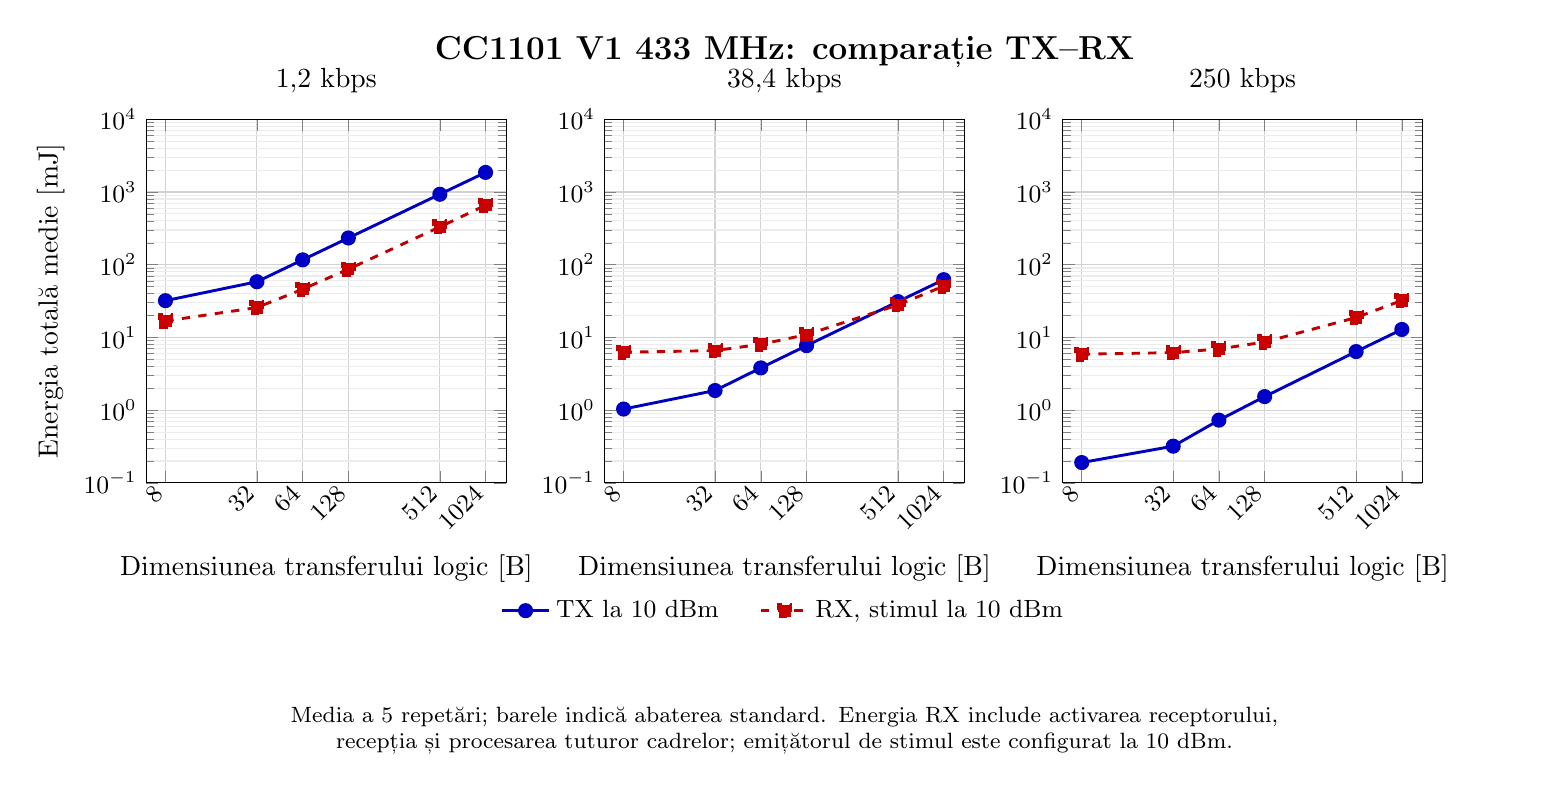
\begin{tikzpicture}
\begin{groupplot}[/pgf/number format/use comma,
  group style={group size=3 by 1, horizontal sep=1.25cm},
  width=6.15cm, height=6.2cm,
  xmode=log, log basis x={2},
  ymode=log, log basis y={10},
  ymin=0.1, ymax=10000,
  xmin=6, xmax=1400,
  xtick={8,32,64,128,512,1024},
  xticklabels={8,32,64,128,512,1024},
  x tick label style={rotate=45, anchor=east, font=\small},
  y tick label style={font=\small},
  grid=both, minor grid style={gray!15}, major grid style={gray!35},
  xlabel={Dimensiunea transferului logic [B]},
  every axis plot/.append style={line width=1.05pt},
  error bars/error bar style={line width=0.35pt},
  legend style={font=\small, draw=none, fill=none,
    at={(0.5,-0.29)}, anchor=north, legend columns=3,
    /tikz/every even column/.append style={column sep=0.45cm}},
]
\nextgroupplot[title={1{,}2 kbps}, ylabel={Energia totală medie [mJ]}]
\addplot+[
  color=blue!75!black, solid, mark=*, mark size=2.2pt,
  error bars/.cd, y dir=both, y explicit,
] coordinates {
  (8,32.0446747) +- (0,0.0370598432)
  (32,58.3144302) +- (0,0.0237579511)
  (64,116.672096) +- (0,0.111018904)
  (128,233.136856) +- (0,0.10288105)
  (512,930.375152) +- (0,0.301867613)
  (1024,1857.92992) +- (0,0.516739194)
};
\addplot+[
  color=red!75!black, dashed, mark=square*, mark size=2.2pt,
  error bars/.cd, y dir=both, y explicit,
] coordinates {
  (8,16.8278816) +- (0,0.120838977)
  (32,25.7746308) +- (0,0.102007568)
  (64,46.0118558) +- (0,0.113464721)
  (128,86.8321499) +- (0,0.147199542)
  (512,330.71195) +- (0,0.193649172)
  (1024,656.739148) +- (0,0.399831612)
};
\nextgroupplot[title={38{,}4 kbps}]
\addplot+[
  color=blue!75!black, solid, mark=*, mark size=2.2pt,
  error bars/.cd, y dir=both, y explicit,
] coordinates {
  (8,1.03566357) +- (0,0.0033639912)
  (32,1.86283151) +- (0,0.00413811507)
  (64,3.81086863) +- (0,0.00510905198)
  (128,7.71433063) +- (0,0.00260353714)
  (512,31.0961076) +- (0,0.00925000582)
  (1024,62.2809748) +- (0,0.00981065808)
};
\addlegendentry{TX la 10 dBm}
\addplot+[
  color=red!75!black, dashed, mark=square*, mark size=2.2pt,
  error bars/.cd, y dir=both, y explicit,
] coordinates {
  (8,6.25459515) +- (0,0.116129769)
  (32,6.59544601) +- (0,0.0791978764)
  (64,8.04293272) +- (0,0.165120793)
  (128,10.9234085) +- (0,0.102236083)
  (512,28.0142939) +- (0,0.129088767)
  (1024,50.7539839) +- (0,0.20347594)
};
\addlegendentry{RX, stimul la 10 dBm}
\nextgroupplot[title={250 kbps}]
\addplot+[
  color=blue!75!black, solid, mark=*, mark size=2.2pt,
  error bars/.cd, y dir=both, y explicit,
] coordinates {
  (8,0.190372885) +- (0,0.00139155929)
  (32,0.31967722) +- (0,0.00209535265)
  (64,0.729163421) +- (0,0.00128311596)
  (128,1.53636609) +- (0,0.00416778569)
  (512,6.38997669) +- (0,0.00765916982)
  (1024,12.8732147) +- (0,0.00806386669)
};
\addplot+[
  color=red!75!black, dashed, mark=square*, mark size=2.2pt,
  error bars/.cd, y dir=both, y explicit,
] coordinates {
  (8,5.89787083) +- (0,0.0638509332)
  (32,6.17719294) +- (0,0.0550834758)
  (64,6.94242591) +- (0,0.0821845355)
  (128,8.64849991) +- (0,0.0854631257)
  (512,18.7823436) +- (0,0.125971716)
  (1024,32.2143987) +- (0,0.105953369)
};
\end{groupplot}
\node[font=\bfseries\large] at ($(group c2r1.north)+(0,0.85cm)$)
  {CC1101 V1 433 MHz: comparație TX--RX};
\node[font=\footnotesize, align=center, text width=18.5cm]
  at ($(group c2r1.south)+(0,-3.15cm)$)
  {Media a 5 repetări; barele indică abaterea standard. Energia RX include activarea receptorului,\\
   recepția și procesarea tuturor cadrelor; emițătorul de stimul este configurat la 10 dBm.};
\end{tikzpicture}
\end{document}
